\progpart
\section{programming: การหารลงตัวที่เขียนกันเองด้วยนิยาม}
\begin{figure}[h]\label{div_sol1}
	\begin{center}
		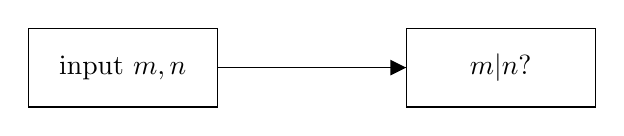
\begin{tikzpicture}[scale=0.2]
			\tikzstyle{every node}+=[inner sep=0pt]
			\draw [black] (0,-2.5) rectangle ++(12,5);
			\draw (6,0) node {input $m,n$};
			\draw [black] (12,0) -- (24,0);
			\fill [black] (24,0) -- (23,0.5) -- (23,-0.5);
			\draw [black] (24,-2.5) rectangle ++(12,5);
			\draw (30,0) node {$m|n$?};
		\end{tikzpicture}
		\caption{ภาพใหญ่ของปัญหาซึ่ง input คือจำนวนนับ $m,n$ และ output คือบอกว่าหารลงตัวหรือไม่}
	\end{center}
\end{figure}
เราจะเริ่มจากนิยามแรกสุดของทฤษฎีจำนวน นั่นคือการหารลงตัวของจำนวนเต็ม ซึ่งจริง ๆ แล้วนั้นเราสามารถตรวจสอบว่าจำนวน 2 จำนวนเช่น $m$ และ $n$ ที่ให้มานั้นหารลงตัวกันหรือไม่ได้โดยง่ายผ่านตัวดำเนินการ ``\%'' ซึ่งเป็นตัวดำเนินการ built-in ของ Python เพื่อหาเศษเหลือจากการหาร โดยตรวจสอบว่าเศษเหลือเป็น 0 หรือไม่ด้วย code ดังนี้
\begin{python*}
m%n == 0
\end{python*}
\noindent โดยที่ code ดังกล่าวจะคืนค่า True ถ้าหารลงตัว และคืนค่า False ถ้าหารไม่ลงตัว

แต่ในที่นี้เราจะเริ่มเขียนฟังก์ชันเพื่อตรวจสอบการหารลงตัวกันด้วยตัวเองก่อนโดยอาศัยนิยามในการออกแบบ โดยสมมติว่าเราจะให้พารามิเตอร์แรกเป็นตัวตั้งและพารามิเตอร์ตัวที่สองเป็นตัวหาร และชื่อฟังก์ชันคือ \texttt{isDivisible} แต่ก่อนจะเริ่มลงมือเขียน code เราจะมาทบทวนนิยามของการหารลงตัวกันอีกรอบ
\boxrule{ทบทวนนิยามการหารลงตัว}{ให้ $m$ และ $n$ เป็นจำนวนเต็ม เราจะกล่าวว่า $m$ หารด้วย $n$ ลงตัว ถ้ามีจำนวนเต็ม $k$ ที่ทำให้ $m=nk$}

จากนิยาม จะเห็นว่าเป้าหมายหลักของฟังก์ชันหลังจากที่รับ $m$ และ $n$ เข้ามาแล้วคือต้องหาว่ามีจำนวนเต็ม $k$ ที่เป็นผลหารดังกล่าวหรือไม่ โดยถ้าดูตามนิยามแล้วจะดูเหมือนว่าเราต้องตรวจสอบหาผลหาร $k$ ไปเรื่อยๆ จนกว่าจะพบ $k$ ที่ทำให้ $m=nk$ ดังนี้
\begin{python*}[Not complete divisibility checking]
k = 1
while m != n*k:
    k += 1
# after exiting from while-loop, k should be an integer such that m = nk,
# i.e. n is a factor of m
\end{python*}
\noindent ทว่า วิธีดังกล่าวจะทำงานไม่รู้จบถ้าค่าที่ได้รับเข้ามาเป็นคู่ที่หารกันไม่ลงตัว เพราะเหตุผลของการหารไม่ลงตัวคือ
\begin{align*}
	m\nmid n
	&\Longleftrightarrow \text{ทุก $k \in \Z$ จะได้ว่า $m \neq nk$}
\end{align*}
กล่าวคือ เราต้องตรวจสอบทุกจำนวนเต็ม $k$ ซึ่งเป็นไปไม่ได้ในการเขียนโปรแกรม อีกทั้ง ถึงแม้ว่าจะหารลงตัวก็ตาม ก็ยังคงมีคำถามว่าแล้วเราจะเริ่มหา $k$ จากไหนและไปทางไหน เพราะถ้าหาผิดทางอาจจะทำงานไม่รู้จบได้เหมือนกัน ตัวอย่างเช่นเราอยากตรวจสอบว่า -10 หารด้วย 5 หรือไม่ ถ้าเราใช้ loop เริ่มจาก $k=1$ และบวก 1 ไปเรื่อย ๆ ดังตัวอย่างข้างบน จะพบว่าโปรแกรมจะทำงานไม่รู้จบเพราะ $k$ ตัวที่ต้องการคือ $k = -2$ ซึ่งไม่อยู่นี้ขอบเขตการหาที่กำหนดไว้

แต่ว่าเรามีคุณสมบัติหนึ่งที่เกี่ยวกับการหารลงตัวที่สามารถจำกัดขอบเขตการหาผลหาร $k$ ได้ ซึ่งกล่าวว่า
\boxrule{คุณสมบัติเพื่อจำกัดขอบเขตของการหารลงตัว}{ให้ $m$ และ $n$ เป็นจำนวนเต็ม ถ้า $m|n$ แล้ว $|n|\leq |m|$}
ซึ่งในทำนองเดียวกัน เราสามารถมองผลหารเป็นตัวประกอบอีกตัวหนึ่งของ $m$ ได้เช่นเดียวกัน จึงได้ว่า $|k| \leq |m|$ กล่าวคือถ้าจะมีผลหารของการหารลงตัวได้นั้น ผลหารดังกล่าวก็จะอยู่ได้แค่ในกลุ่ม $k\in \{-m, -m+1, \dots, -1,0,1, \dots, m-1, m\}$ เพราะฉะนั้น เราจึงจำกัดขอบเขตการหาผลหาร $k$ ได้ไม่ว่าจะหารลงตัวหรือหารไม่ลงตัวก็ตาม กล่าวคือ
\begin{align*}
	m | n
	&\Longleftrightarrow \text{มี $k \in \{-m, -m+1, \dots, m-1, m\}$ ที่ทำให้ $m = nk$}
\end{align*}

\subsection{วิธีเบื้องต้น}
จากนิยามที่ได้กล่าวมานั้น เราสามารถเขียนโปรแกรมเพื่อตรวจสอบการหารลงตัวได้ด้วยการตรวจสอบว่าเจอผลหารหรือไม่ด้วยโปรแกรมดังนี้
\begin{python*}[Check divisibility]
def isDivisible_ver1(m,n):
    qoutList = range(-m,m+1)
    for k in qoutList:
        if m = n*k:
            return True
    return False
\end{python*}
ซึ่งโปรแกรมดังกล่าวจะรันลูปไปเรื่อย ๆ และเมื่อไหร่ก็ตามที่เจอผลหาร ฟังก์ชัน isDivisible จะคืนค่า True มาให้ แต่ถ้ารันจนครบลูปแล้วแต่ไม่เจอผลหาร จะคืนค่า False มาให้ เพราะไม่มีตัวประกอบ
\boxrule{ลองทำดู}{ออกแบบให้จำนวนครั้งการค้นหาลดลงได้หรือไม่ ถ้าทำได้แล้วความซับซ้อนของจำนวนครั้งการค้นหาลดลงหรือไม่}

\subsection{พิจารณาแค่จำนวนบวกก็พอ}
ถ้าลองสังเกตนิยามการหารลงตัวดีๆ จะพบว่าการเป็นจำนวนเต็มบวกหรือจำนวนเต็มลบของตัวตั้งและตัวหารไม่ส่งผลต่อการคิด เพราะเราสามารถเปลี่ยนรูปแบบปัญหาให้พิจารณาแค่กรณีที่ทั้งตัวตั้งและตัวหารเป็นจำนวนเต็มบวกอย่างเดียวได้ เนื่องจากถ้า $m = nk$ แล้วจะได้ว่า
\begin{align*}
	(-m) = nk &\Longleftrightarrow m = n(-k)\\
	m = (-n)k &\Longleftrightarrow m = n(-k)\\
	(-m) = (-n)k &\Longleftrightarrow m = nk
\end{align*}
กล่าวคือ เราทราบการเป็นบวกหรือลบของผลหาร $k$ ได้โดยพิจารณาก่อนว่าตัวตั้งและตัวหารมีเครื่องเหมือนกันหรือแตกต่างกัน และใช้การตรวจสอบการหารลงตัวโดยอาศัยแค่ค่าบวกของ $m$ และ $n$ ที่เป็นตัวตั้งและตัวหาร

แต่เนื่องจากเราต้องการผลลัพธ์ในแง่การหารลงตัวว่าหารลงตัวหรือไม่ ไม่ได้ต้องการค่าผลหาร จึงไม่จำเป็นต้องแบ่งกรณีการคำนวณของโปรแกรมออกตามความเหมือนหรือความต่างของเครื่องหมายของตัวตั้งและตัวหาร กล่าวคือเราสามารถพิจารณาแค่ค่าบวกของทั้งคู่และตัดขอบเขตการหาผลลัพธ์การหารเป็นแค่ $k\in \{1,2, \dots, m-1, m\}$ ซึ่งจะได้โปรแกรมดังนี้
\begin{python*}[Check divisibility by positive]
def isDivisible_ver2(m,n):
    if m < 0:
        m = -m
    if n < 0:
        n = -n
    qoutList = range(1,m+1)
    for k in qoutList:
        if m = n*k:
            return True
    return False
\end{python*}
และโปรแกรมสำหรับการตรวจสอบการหารลงตัวที่จะพัฒนาต่อจากนี้จะขอสมมติว่าเรารับแค่จำนวนเต็มบวกมาตรวจสอบ ซึ่งถ้าจะทำให้รับจำนวนเต็มใด ๆ สามารถทำได้ในทำนองเดียวกันกับ \texttt{isDivisible\_ver2}

\subsection{เปลี่ยนจากปัญหาการคูณเป็นปัญหาการบวก}
จากนิยามการคูณที่กล่าวว่า $k\cdot n := n + n + \cdots + n$ ($k$ พจน์) จะพบว่าเราสามารถเปลี่ยนจากปัญหาการหาผลหาร $k$ เป็นการลองลูปเพื่อเพิ่มพจน์การบวก $n$ ไปเรื่อย ๆ จนกว่าจะมากกว่าหรือเท่ากับ $m$ โดยถ้าสามารถเท่ากับ $m$ ได้จะได้ว่าหารลงตัว แต่ถ้าเกิน $m$ เมื่อไหร่จะได้ว่าหารไม่ลงตัว
\begin{python*}[Check divisibility addition version]
def isDivisible_ver3(m,n):
    product = 0
    while product < m:
        product += n
    if product == m:
        return True
    else:
        return False
\end{python*}
เราสามารถทำได้ในทางกลับกันคือการลบตัวหารออกด้วย $n$ ไปเรื่อยๆ จนกว่าจะได้เศษการหาร (ซึ่งนำไปประยุกต์ใช้ในการหาเศษการหารได้ด้วย)
\begin{python*}[Check divisibility subtraction version]
def isDivisible_ver4(m,n):
    while m >= n:
        m -= n
    if m == 0:
        return True
    else:
        return False
\end{python*}

\subsection{เขียนแบบฟังก์ชันเวียนเกิด} \label{divisibleRecur}
จาก \texttt{isDivisible\_ver4} จะเห็นแนวคิดของการทำปัญหาเดิมซ้ำกัน โดยถ้าเริ่มจากตัวตั้ง $m$ และตัวหาร $n$ เมื่อทำเสร็จไป 1 รอบของลูป จะได้ว่าตัวตั้งจะเปลี่ยนกลายเป็น $m - n$ โดยที่ตัวหารยังคง $n$ เหมือนเดิม ซึ่งจะเห็นว่าแนวคิดดังกล่าวสามารถเขียนเป็นฟังก์ชันเวียนเกิดเป็น \[ \texttt{isDivisible\_recur(m,n)} = \texttt{isDivisible\_recur(m - n,n)} \]
และตามรูปแบบการเขียนอัลกอริทึมเวียนเกิด สิ่งสำคัญคือต้องเขียนขั้นฐานของการคำนวณ ซึ่งคือขั้นที่เราสามารถกำหนดการคำนวณได้ง่าย ๆ โดยจะพบว่า ขั้นฐานของการคำนวณคือขั้นตอนหลังจากหลุดออกจาก while-loop ของ \texttt{isDivisible\_ver4} กล่าวคือ เมื่อตัวตั้ง $m$ ไม่ค่าน้อยกว่าตัวหาร $n$ โดยที่ถ้าตัวตั้งมีค่าเท่ากับ 0 จะหมายความว่าเราสามารถลดค่าตัวตั้งมาเรื่อย ๆ จนหมดได้พอดี หรือก็คือมีเศษเหลือเป็น 0 นั่นคือการหารลงตัว ในทางกลับกัน ถ้าตัวตั้งมีค่ามากกว่า 0 จะหมายถึงการหารไม่ลงตัว ซึ่งสามารถเขียนเป็นเงื่อนไขขั้นฐานได้ดังนี้ \[ \texttt{isDivisible\_recur(m,n)} = \begin{cases}	\texttt{True}&\text{if }m=0\\
\texttt{False}&\text{if }0<m<n
\end{cases}
\] ซึ่งสามารถเขียนเป็นโปรแกรมได้ดังนี้
\begin{python*}[Check divisibility recursion]
def isDivisible_recur(m,n):
    if m < n:
        if m == 0:
            return True
        else:
            return False
    else:
        return isDivisible_recur(m-n,n)
\end{python*}






\newpage
\section{programming: ตรวจสอบการเป็นจำนวนเฉพาะ}
\subsection{วิธีเบื้องต้น}
ในหัวข้อที่แล้ว เราได้เขียนฟังก์ชันเพื่อตรวจสอบการหารลงตัวไป ในหัวข้อนี้เราจะใช้ประโยชน์จากฟังก์ชันดังกล่าวนำมาตรวจสอบการเป็นจำนวนเฉพาะกันบ้าง โดยลักษณะของปัญหายังคงตรงไปตรงมาคือรับจำนวนนับ $n$ เข้ามาแล้วคืนค่าว่าเป็นจำนวนเฉพาะหรือไม่ดังแผนภาพใน Figure \ref{prime_sol1}
\begin{figure}[h]\label{prime_sol1}
\begin{center}
	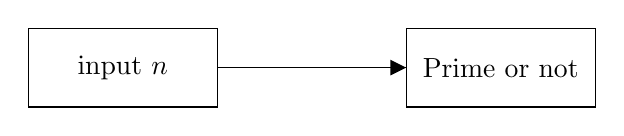
\begin{tikzpicture}[scale=0.2]
		\tikzstyle{every node}+=[inner sep=0pt]
		\draw [black] (0,-2.5) rectangle ++(12,5);
		\draw (6,0) node {input $n$};
		\draw [black] (12,0) -- (24,0);
		\fill [black] (24,0) -- (23,0.5) -- (23,-0.5);
		\draw [black] (24,-2.5) rectangle ++(12,5);
		\draw (30,0) node {Prime or not};
		
	\end{tikzpicture}
	\caption{ภาพใหญ่ของปัญหาซึ่ง input คือจำนวนนับ $n$ และ output คือบอกว่าเป็นจำนวนเฉพาะหรือไม่}
\end{center}
\end{figure}

เริ่มจากทบทวนนิยามของจำนวนเฉพาะ ซึ่งคือ
\boxrule{ทบทวนนิยามจำนวนเฉพาะ}{จำนวนนับ $n$ จะเป็นจำนวนเฉพาะ ถ้ามีเพียงแค่ 1 และ $n$ เท่านั้นที่หาร $n$ ลงตัว}
ซึ่งจากนิยามจะพบว่าเราสามารถตรวจสอบการเป็นจำนวนเฉพาะได้จากการตรวจสอบการหารลงตัวว่าในช่วงตั้งแต่ 1 ถึงจำนวนดังกล่าวมีเพียงแค่ 1 และตัวมันเองเท่านั้นที่หารจำนวนดังกล่าวลงตัว กล่าวคือถ้าเราหาตัวประกอบทั้งหมดของ $n$ ได้ แล้วทำการตรวจสอบว่าเป็นจำนวนเฉพาะหรือไม่ก็จะสามารถตรวจสอบการเป็นจำนวนเฉพาะของ $n$ ได้ทันทีตามแผนภาพใน Figure \ref{prime_sol2}
\begin{figure}[h]\label{prime_sol2}
\centering
		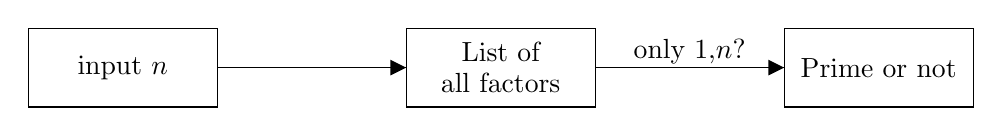
\begin{tikzpicture}[scale=0.2]
			\tikzstyle{every node}+=[inner sep=0pt]
			
			\draw [black] (0,-2.5) rectangle ++(12,5);
			\draw (6,0) node {input $n$};
			\draw [black] (12,0) -- (24,0);
			\fill [black] (24,0) -- (23,0.5) -- (23,-0.5);
			\draw [black] (24,-2.5) rectangle ++(12,5);
			\draw (30,1) node {List of};
			\draw (30,-1) node {all factors};
			
			\draw [black] (36,0) -- (48,0);
			\draw (42,1) node {only 1,$n$?};
			\fill [black] (48,0) -- (47,0.5) -- (47,-0.5);
			\draw [black] (48,0-2.5) rectangle ++(12,5);
			\draw (54,0) node {Prime or not};
		\end{tikzpicture}
		\caption{text}
\end{figure} 
ซึ่่งถ้าเรามีลิสต์ของตัวประกอบของ $n$ แล้วเราจะสามารถเขียนโค้ดเพื่อตรวจสอบการเป็นจำนวนเฉพาะได้ดังนี้
\begin{python*}[Check if it is prime]
# assume we have a list `factorList` which is a list of all factors of n
factorList == [1,n]
\end{python*}

ซึ่งโค้ดดังกล่าวจะให้ค่า True ออกมาถ้า $n$ มีตัวประกอบเพียงแค่ 2 ตัวคือ 1 และ $n$ กล่าวคือ $n$ เป็นจำนวนเฉพาะ แต่ในทางกลับกัน ถ้ามีตัวประกอบอื่นหลงอยู่ในลิสต์ดังกล่าวซึ่งก็คือ $n$ ไม่เป็นจำนวนเฉพาะนั้น จะได้ False ออกมาเป็นผลลัพธ์

\begin{figure}[h]\label{prime_sol3}
	\centering
	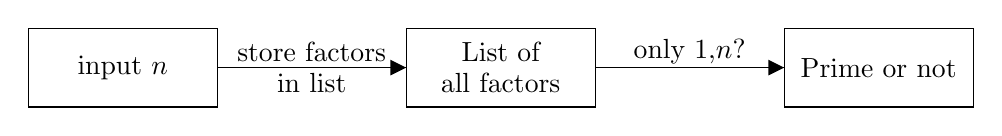
\begin{tikzpicture}[scale=0.2]
		\tikzstyle{every node}+=[inner sep=0pt]
		\draw [black] (0,-2.5) rectangle ++(12,5);
		\draw (6,0) node {input $n$};
		\draw [black] (12,0) -- (24,0);
		\fill [black] (24,0) -- (23,0.5) -- (23,-0.5);
		\draw [black] (24,-2.5) rectangle ++(12,5);
		\draw (30,1) node {List of};
		\draw (30,-1) node {all factors};
		
		\draw [black] (36,0) -- (48,0);
		\draw (42,1) node {only 1,$n$?};
		\fill [black] (48,0) -- (47,0.5) -- (47,-0.5);
		\draw [black] (48,0-2.5) rectangle ++(12,5);
		\draw (54,0) node {Prime or not};
		\draw (18,1) node {store factors};
		\draw (18,-1) node {in list};
	\end{tikzpicture}
	\caption{text}
\end{figure} 

ในตอนนี้เราจะเหลือเพียงแค่ปัญหาของการสร้างลิสต์ของตัวประกอบของ $n$ ซึ่งทำได้โดยง่าย (ใน Python) โดยการรันลูปตั้งแต่ 1 ถึง $n$ และตรวจสอบการเป็นตัวประกอบของ $n$ เพื่อนำไปเก็บใน \texttt{factorList} ทีละตัว ซึ่งทำได้ดังนี้

\begin{python*}[Create factorList]
factorList = []
for m in range(1,n+1):
    if isDivisible(n,m):
        factorList.append(m)
\end{python*}

เมื่อนำโค้ดทั้งสองส่วนมารวมกันและเขียนเป็นฟังก์ชันของ $n$ จะได้
\begin{python}[Check prime]
def isPrime(n):

    factorList = []
    for m in range(1,n+1):
        if isDivisible(n,m):
            factorList.append(m)

    prime = (factorList == [1,n])
    return prime
\end{python}

ทั้งนี้ ยังคงมีคำถามชวนคิดเกี่ยวกับโปรแกรมเช็คจำนวนเฉพาะที่เขียนขึ้นมาว่า
\boxrule{คำถาม}{เพราะเหตุใดเราจึงเขียนลูปแค่บน 1 ถึง $n$ ก็เพียงพอที่จะเช็คการเป็นจำนวนเฉพาะของ $n$ ได้}

จากโปรแกรมที่เขียนมา จะเห็นว่าเราใช้พลังของการมี memory กล่าวคือเราเก็บไว้ก่อนว่ามีใครบ้างเป็นตัวประกอบ แล้วสุดท้ายนำมาตรวจสอบอีกทีว่ามีแค่ 1 และตัวมันเองเท่านั้นที่เป็นตัวประกอบ ซึ่งเราทำการเก็บตัวประกอบไว้ในลิสต์ ซึ่งเป็นเรื่องที่โชคดีที่ลิสต์เป็น built-in data structure ของ Python จึงทำให้เราสามารถ implement วิธีนี้ได้โดยง่าย
ทว่า ในบางภาษานั้นกลับไม่มีลิสต์ให้ใช้ และการตรวจสอบเรื่องการมีใครเป็นสมาชิกบ้างก็ไม่ใช่เรื่องง่ายกับ array ที่เป็นโครงสร้างข้อมูลพื้นฐานในหลาย ๆ ภาษา
ดังนั้น จะแก้ปัญหาอย่างไรถ้าเราอยาก implement โจทย์นี้ในภาษาอื่น ๆ หรือแม้กระทั่งในวิชา Python เองแต่ยังเรียนไม่ถึงการใช้ลิสต์

\subsection{วิธีที่ไม่ใช้ลิสต์ หรือการจำตัวประกอบทั้งหมดของ $n$}
ก่อนอื่น เราจะต้องเปลี่ยนรูปแบบปัญหาให้เป็นปัญหาทางตรรกศาสตร์กันก่อน โดยเริ่มจากนิยามกัน
\begin{align*}
	n>1 \text{ เป็นจำนวนเฉพาะ}
	&\Longleftrightarrow \text{มีเพียงแค่ 1 และ $n$ ที่เป็นตัวประกอบของ $n$}\\
	&\Longleftrightarrow \text{ถ้า $k \notin \{1,n\}$ แล้ว $k$ จะไม่เป็นตัวประกอบของ $n$}\\
	&\Longleftrightarrow \text{ทุก $k=2,...,n-1$ จะได้ว่า $k$ ไม่เป็นตัวประกอบของ $n$}
\end{align*}
หรือในทำนองเดียวกัน เพียงแต่ใช้ความสมมูลเชิงนิเสธ จะได้ว่า
\begin{align*}
	n>1 \text{ ไม่เป็นจำนวนเฉพาะ}
	&\Longleftrightarrow \text{มี $k=2,...,n-1$ ที่ $k$ เป็นตัวประกอบของ $n$}
\end{align*}

กล่าวคือ ถ้าเราจะตรวจสอบว่า $n$ ไม่เป็นจำนวนเฉพาะ เราสามารถทำได้ โดยลูปตั้งแต่ 2 ถึง $n-1$ และเมื่อใดก็ตามที่เจอตัวประกอบเพียงสักตัว เราก็จะสามารถหยุดลูปและบอกได้ทันทีว่า $n$ ไม่เป็นจำนวนเฉพาะ (มาจากการให้เหตุผลว่าประพจน์ $\exists x, P(x)$ เป็นจริง) ซึ่งทำให้เราสามารถเขียนโค้ดได้ดังนี้

\begin{python}[Check prime version2]
def isPrime_ver2(n):

    prime = True               #set as default to be prime
    for k in range(2,n):
        if isDivisible(n,k):   #check if factor
            prime = False      #if k is a factor, set it to be not prime
            break              #stop for loop
    
    return prime
\end{python}

\boxrule{แบบฝึกหัดเพิ่ม}{ลองเขียน \texttt{isPrime\_ver3} โดยใช้ while-loop}
~
\subsection{ลดจำนวนครั้งการคำนวณได้มากกว่านี้อีก}
จากโปรแกรมที่ได้ทำมาแล้วนั้น เราจะพบว่า \texttt{isPrime} มีความซับซ้อนเชิงคำนวณอยู่ที่ $O(n)$ และ \texttt{isPrime\_ver2} มีความซับซ้อนเชิงการคำนวณไม่เกิน $O(n)$ ซึ่งกรณีแย่ที่สุดคือ $n$ ที่เป็นจำนวนเฉพาะ เพราะต้องตรวจสอบทุกจำนวนตั้งแต่ 2 ถึง $n-1$ ว่าเป็นตัวประกอบหรือไม่

ทว่า เราสามารถอาศัยทฤษฎีบทเกี่ยวกับจำนวนเฉพาะที่กล่าวว่า
\boxrule
{การตรวจสอบการเป็นจำนวนเฉพาะโดยตรวจสอบไม่เกิน $\sqrt{n}$ ครั้ง}
{ให้ $n$ เป็นจำนวนนับ ถ้า $p$ ไม่เป็นตัวประกอบของ $n$ สำหรับทุก ๆ จำนวนเฉพาะ $p\leq \sqrt{n}$ แล้ว $n$ จะเป็นจำนวนเฉพาะ}
ถึงแม้ทฤษฎีบทจะบอกว่าเพียงพอที่จะตรวจสอบแค่ตัวประกอบที่เป็นจำนวนเฉพาะที่มีค่าไม่เกิน $\sqrt{n}$ แต่ว่าในการพิจารณากับแค่จำนวน $n$ เพียงจำนวนเดียว เราจะยังคงไม่มีข้อมูลเก่าว่าจำนวนใดบ้างที่เป็นจำนวนเฉพาะ ดังนั้นวิธีที่ง่ายที่สุดคือตรวจสอบกับทุกจำนวนตั้งแต่ 2 ถึง $\lfloor\sqrt{n}\rfloor$ ว่ามีใครบ้างที่เป็นตัวประกอบของ $n$ ซึ่งทำให้เราสามารถแก้โค้ด \texttt{isPrime\_ver2} ให้ตรวจสอบน้อยลงได้ดังนี้

\begin{python}[Check prime version2.1]
import math
def isPrime_ver2_1(n):
    prime = True               #set as default to be prime
    upper = int(math.sqrt(n))
    for k in range(2,upper):
        if isDivisible(n,k):   #check if factor
            prime = False      #if k is a factor, set it to be not prime
            break              #stop for loop
    return prime
\end{python}

\section{programming: แยกตัวประกอบในรูปผลคูณจำนวนเฉพาะ} \label{primeFactor}
หนึ่งในทฤษฎีบทสำคัญของการแยกตัวประกอบของจำนวนเต็มคือ Fundamental Theorem of Arithmetic ซึ่งกล่าวว่า
\boxrule{Fundamental Theorem of Arithmetic}{
	ทุก ๆ จำนวนเต็ม $n$ จะมีจำนวนเฉพาะ $p_1 < p_2 < \dots < p_n$ และจำนวนเต็มบวก $a_1, a_2, \dots, a_n$ เพียงชุดเดียวเท่านั้นที่ทำให้
	$$
	n = p_1^{a_1}p_2^{a_2}\cdots p_n^{a_n}
	$$
	}
ซึ่งเราได้ศึกษาและพิสูจน์ไปแล้วในหัวข้อ \ref{...}

ในหัวข้อนี้ เราจะเขียนโปรแกรมเพื่อหารูปแบบนี้กัน โดยสมมติว่าเราอยากให้โปรแกรมคืนค่าออกมาเป็น dictionary ที่มี keys ระบุจำนวนเฉพาะ และ values ระบุเลขชี้กำลัง ตัวอย่างเช่น $1400=2^3\times 5^2 \times 7$ จะให้ผลลัพธ์ออกมาเป็น \texttt{\{2:3, 5:2, 7:1\}}
\begin{figure}[H]\label{primeFac_sol1}
	\begin{center}
		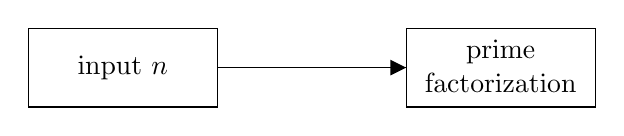
\begin{tikzpicture}[scale=0.2]
			\tikzstyle{every node}+=[inner sep=0pt]
			\draw [black] (0,-2.5) rectangle ++(12,5);
			\draw (6,0) node {input $n$};
			\draw [black] (12,0) -- (24,0);
			\fill [black] (24,0) -- (23,0.5) -- (23,-0.5);
			\draw [black] (24,-2.5) rectangle ++(12,5);
			\draw (30,1) node {prime};
			\draw (30,-1) node {factorization};
		\end{tikzpicture}
		\caption{ภาพใหญ่ของปัญหาซึ่ง input คือจำนวนนับ $n$ และ output คือการแยกตัวประกอบจำนวนเฉพาะที่คืนค่าออกมาเป็น dictionary}
	\end{center}
\end{figure}

\subsection{วิธีวนซ้ำตามจำนวนเฉพาะ}
\subsubsection{ขั้นตอนทำความเข้าใจปัญหา}
จากรูปแบบปัญหา จะเห็นได้โดยง่ายว่าวิธีที่พื้นฐานที่สุดที่ทำได้คือการวนซ้ำไปตามตัวประกอบจำนวนเฉพาะเพื่อหาว่าจะสามารถแยกตัวประกอบจำนวนเฉพาะนั้นออกมาได้กี่รอบ กล่าวคือเราสามารถแยกย่อยปัญหาดังกล่าวออกมาเป็นปัญหาย่อยของทีละจำนวนเฉพาะที่เป็นตัวประกอบ โดยเป็นโจทย์ย่อยว่า

\begin{center}
	กำหนดจำนวนนับ $n$ และจำนวนเฉพาะ $p$\\
	เขียนโปรแกรมเพื่อหาว่าสามารถแยกตัวประกอบ $p$ นั้นออกมาได้กี่ตัว\\
	พูดอีกนัยหนึ่งคือ จงหาจำนวนนับ $k$ ที่ทำให้ $n = p^k\cdot A$ โดยที่ $p\nmid A$
\end{center}

\noindent และเขียนแผนภาพการแก้ปัญหาได้แบบแแผนภาพ \ref{primeFac_sol2}
\begin{figure}[H]
	\begin{center}
		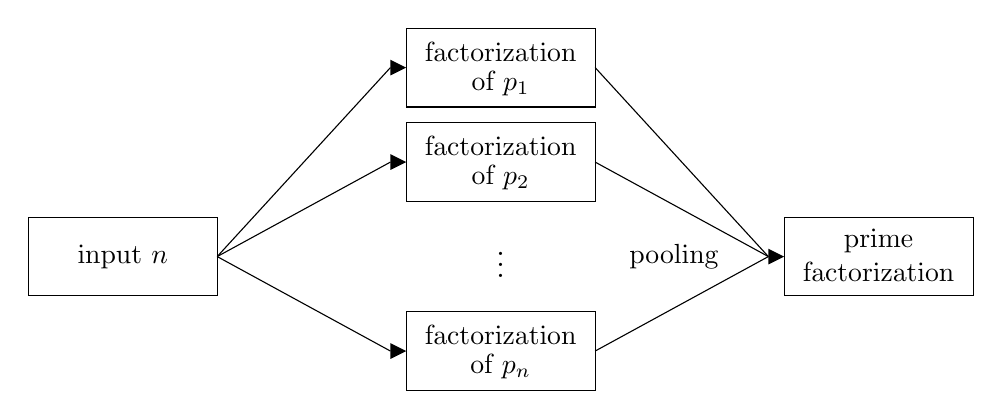
\begin{tikzpicture}[scale=0.2]
			\tikzstyle{every node}+=[inner sep=0pt]
			\draw [black] (0,-2.5) rectangle ++(12,5);
			\draw (6,0) node {input $n$};
			
			\draw [black] (24,-8.5) rectangle ++(12,5);
			\draw [black] (12,0) -- (23,-6);
			\fill [black] (24,-6) -- (23,-5.5) -- (23,-6.5);
			\draw (30,-5) node {factorization};
			\draw (30,-7) node {of $p_n$};
			
			\draw (30,0) node {{\large $\vdots$}};
			\draw [black] (24,3.5) rectangle ++(12,5);
			\draw [black] (12,0) -- (23,6);
			\fill [black] (24,6) -- (23,5.5) -- (23,6.5);
			\draw (30,7) node {factorization};
			\draw (30,5) node {of $p_2$};
			
			\draw [black] (24,9.5) rectangle ++(12,5);
			\draw [black] (12,0) -- (23,12);
			\fill [black] (24,12) -- (23,12.5) -- (23,11.5);
			\draw (30,13) node {factorization};
			\draw (30,11) node {of $p_1$};
			
			\draw [black] (47,0) -- (36,12);
			\draw [black] (47,0) -- (36,6);
			\draw [black] (47,0) -- (36,-6);
			\draw (41,0) node {pooling};
			\fill [black] (48,0) -- (47,0.5) -- (47,-0.5);
			\draw [black] (48,-2.5) rectangle ++(12,5);
			\draw (54,1) node {prime};
			\draw (54,-1) node {factorization};
		\end{tikzpicture}
		\caption{...}\label{primeFac_sol2}
	\end{center}
\end{figure}

ทว่า จะพบว่ายังเหลือปัญหาย่อยที่ว่ามีจำนวนเฉพาะใดบ้างที่เป็นตัวประกอบของ $n$ เพื่อที่จะระบุขอบเขตการแก้ปัญหาย่อย $p_1,\dots,p_n$ ดังนั้นก่อนที่จะแก้ปัญหาย่อยการแยกตัวประกอบจำนวนเฉพาะที่กำหนดตัวประกอบจำนวนเฉพาะมาแล้วนั้น เราจะต้องแก้ปัญหาการหาตัวประกอบที่เป็นจำนวนเฉพาะทั้งหมดของ $n$ ก่อน จึงได้แผนภาพการแก้ปัญหาดังแผนภาพ \ref{primeFac_sol3}

\begin{figure}[H]
	\begin{center}
		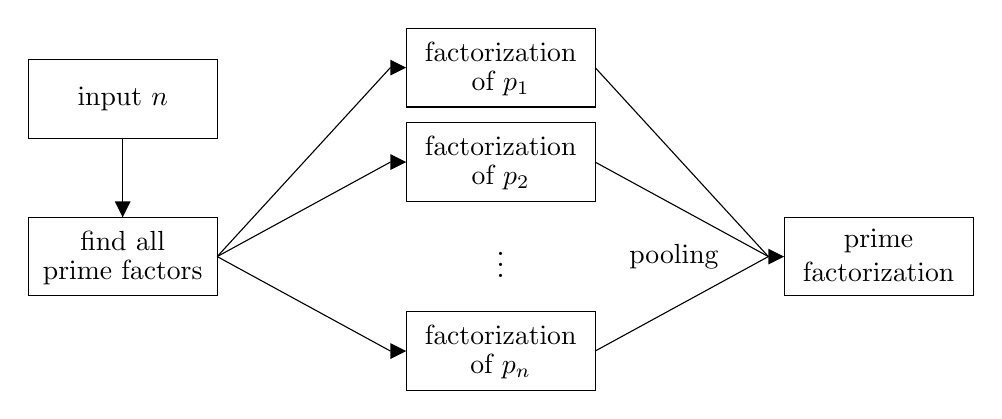
\begin{tikzpicture}[scale=0.2]
			\tikzstyle{every node}+=[inner sep=0pt]
			\draw (6,10) node {input $n$};
			\draw [black] (0,-2.5) rectangle ++(12,5);
			\draw (6,1) node {find all};
			\draw (6,-1) node {prime factors};
			\draw [black] (0,7.5) rectangle ++(12,5);
			\draw [black] (6,7.5) -- (6,2.5);
			\fill [black] (6,2.5) -- (5.5,3.5) -- (6.5,3.5);
			\draw [black] (24,-8.5) rectangle ++(12,5);
			\draw [black] (12,0) -- (23,-6);
			\fill [black] (24,-6) -- (23,-5.5) -- (23,-6.5);
			\draw (30,-5) node {factorization};
			\draw (30,-7) node {of $p_n$};
			
			\draw (30,0) node {{\large $\vdots$}};
			\draw [black] (24,3.5) rectangle ++(12,5);
			\draw [black] (12,0) -- (23,6);
			\fill [black] (24,6) -- (23,5.5) -- (23,6.5);
			\draw (30,7) node {factorization};
			\draw (30,5) node {of $p_2$};
			
			\draw [black] (24,9.5) rectangle ++(12,5);
			\draw [black] (12,0) -- (23,12);
			\fill [black] (24,12) -- (23,12.5) -- (23,11.5);
			\draw (30,13) node {factorization};
			\draw (30,11) node {of $p_1$};
			
			\draw [black] (47,0) -- (36,12);
			\draw [black] (47,0) -- (36,6);
			\draw [black] (47,0) -- (36,-6);
			\draw (41,0) node {pooling};
			\fill [black] (48,0) -- (47,0.5) -- (47,-0.5);
			\draw [black] (48,-2.5) rectangle ++(12,5);
			\draw (54,1) node {prime};
			\draw (54,-1) node {factorization};
		\end{tikzpicture}
		\caption{...}\label{primeFac_sol3}
	\end{center}
\end{figure}

ซึ่งปัญหาย่อยของการแยกตัวประกอบของแต่ละตัวประกอบเฉพาะนั้น เราสามารถใช้ for-loop เพื่อลูปการแก้ปัญหาตามตัวประกอบเฉพาะทั้งหมดที่หามาได้และเก็บผลลัพธ์มาสะสมไว้ ซึ่งจะได้ดังแผนภาพ \ref{primeFac_sol4}
\begin{figure}[H]
	\begin{center}
		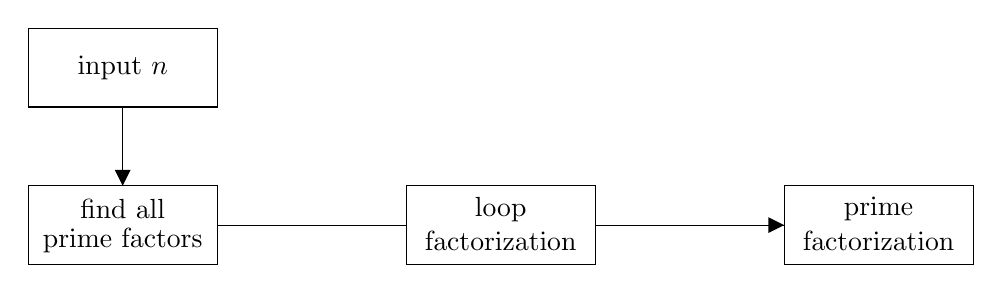
\begin{tikzpicture}[scale=0.2]
			\tikzstyle{every node}+=[inner sep=0pt]
			\draw (6,10) node {input $n$};
			\draw [black] (0,-2.5) rectangle ++(12,5);
			\draw (6,1) node {find all};
			\draw (6,-1) node {prime factors};
			\draw [black] (0,7.5) rectangle ++(12,5);
			\draw [black] (6,7.5) -- (6,2.5);
			\fill [black] (6,2.5) -- (5.5,3.5) -- (6.5,3.5);
			\draw [black] (12,0) -- (24,0);
			\draw [black] (24,-2.5) rectangle ++(12,5);
			\draw (30,1) node {loop};
			\draw (30,-1) node {factorization};
			\draw [black] (36,0) -- (48,0);
			\fill [black] (48,0) -- (47,0.5) -- (47,-0.5);
			\draw [black] (48,-2.5) rectangle ++(12,5);
			\draw (54,1) node {prime};
			\draw (54,-1) node {factorization};
		\end{tikzpicture}
		\caption{...}\label{primeFac_sol4}
	\end{center}
\end{figure}

ทั้งนี้ โจทย์ปัญหาของการหาตัวประกอบที่เป็นจำนวนเฉพาะทั้งหมดของ $n$ จะทิ้งไว้ให้ผู้อ่านทำเป็นแบบฝึกหัดในแบบฝึกหัด \ref{allPrimeFactor} แต่เราจะมาแก้ปัญหาเรื่องจำนวนครั้งการเป็นตัวประกอบของตัวประกอบเฉพาะที่กำหนดมาให้กัน

\subsubsection{แก้ปัญหาย่อยจำนวนครั้งการหารลงตัว}
ก่อนลงรายละเอียด จะขอทบทวนปัญหาอีกสักครั้ง
\begin{center}
	กำหนดจำนวนนับ $n$ และจำนวนเฉพาะ $p$\\
	เขียนโปรแกรมเพื่อหาว่าสามารถแยกตัวประกอบ $p$ นั้นออกมาได้กี่ตัว\\
	พูดอีกนัยหนึ่งคือ จงหาจำนวนนับ $k$ ที่ทำให้ $n = p^k\cdot A$ โดยที่ $p\nmid A$
\end{center}
\begin{figure}[H]\label{subPrimeFac_sol1}
	\begin{center}
		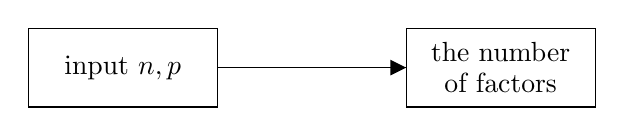
\begin{tikzpicture}[scale=0.2]
			\tikzstyle{every node}+=[inner sep=0pt]
			\draw [black] (0,-2.5) rectangle ++(12,5);
			\draw (6,0) node {input $n, p$};
			\draw [black] (12,0) -- (24,0);
			\fill [black] (24,0) -- (23,0.5) -- (23,-0.5);
			\draw [black] (24,-2.5) rectangle ++(12,5);
			\draw (30,1) node {the number};
			\draw (30,-1) node {of factors};
		\end{tikzpicture}
		\caption{ภาพใหญ่ของปัญหาย่อยซึ่ง input คือจำนวนนับ $n$ และจำนวนเฉพาะ $p$ และ output คือจำนวนครั้งการหาร $n$ ลงตัวของ $p$}
	\end{center}
\end{figure}
ปัญหานี้เป็นปํญหาที่ค่อนข้างง่าย เราสามารถทำได้ด้วยการวนลูปหารซ้ำไปเรื่อย ๆ ด้วยเงื่อนไขว่า ``ตราบใดที่ยังหารลงตัวอยู่ (\texttt{n\%p == 0}) ให้หารต่อ'' และทุกครั้งการหารเราจะมีตัวแปรเพื่อเก็บจำนวนครั้งการหารไว้ (\texttt{counter += 1}) และอัพเดตตัวตั้งการหารเป็นผลหารล่าสุด \texttt{n = n//p} ซึ่งสามารถเขียนเป็นโค้ดได้ดังนี้
\begin{python*}[factorization of given prime $p$]
def countFactor(n,p):
    count = 0
    while n%p == 0:
        count += 1
        n = n//p
    return count
\end{python*}

\subsubsection{รวบรวมวิธีแก้ปัญหาย่อยเพื่อแก้ปัญหาหลัก}
ตอนนี้เรามีฟังก์ชัน \texttt{countFactor} เพื่อช่วยในการนับจำนวนตัวประกอบเฉพาะ $p$ ของ $n$ และ(สมมติ)มีฟังก์ชัน \texttt{findAllPrimeFactor} เพื่อช่วยในการหาตัวประกอบเฉพาะทั้งหมดของ $n$ หรือพูดอีกนัยหนึ่งคือ เราสามารถหาได้แล้วว่าเมื่อทำการแยกตัวประกอบเฉพาะของ $n$ จะมีจำนวนเฉพาะใดคูณกันอยู่บ้าง และแต่ละจำนวนเฉพาะดังกล่าวมีเลขชี้กำลังเป็นอะไร ตอนนี้เหลือเพียงแค่นำ 2 ฟังก์ชันดังกล่าวมาทำงานร่วมกันตามแผนที่วางไว้ในแผนภาพ \ref{primeFac_sol4} ซึ่งเราจะสามารถเขียนโค้ดได้ดังนี้
\begin{python}[Prime Factorization]
def primeFactorize(n):
    primeList = findAllPrimeFactor(n)
    resultDict = {}
    for p in primeList:
        resultDict[p] = countFactor(n,p)
    return resultDict
\end{python}

\subsection{วิธีเวียนเกิด}
ถ้าลองสังเกตวิธีคำนวณของฟังก์ชัน \texttt{countFactor} ดี ๆ จะพบว่ามีแนวคิดของการเรียกฟังก์ชันแบบเวียนเกิดที่สำคัญอยู่อย่างหนึ่ง ซึ่งคือการที่เราไม่ได้พิจารณาตัวตั้งของการหารว่ามีค่า $n$ ที่รับมาตลอดเวลา แต่ $n$ ในการพิจารณารอบถัดไปก็เกิดจากการที่เราตัดทอนตัวประกอบที่หาพบมาแล้วหนึ่งตัว ($n/p$) ซึ่งถึงแม้ว่าในฟังก์ชันดังกล่าวจะทำอยู่กับแค่ $p$ ตัวเดียว แต่เราก็สามารถขยายแนวคิดนี้มาสู่กรณีใด ๆ ที่ไม่ได้กำหนดตัวประกอบเฉพาะตายตัวไว้ได้เช่นกัน

จากประเด็นดังกล่าว จึงนำมาสู่แนวคิดการออกแบบในรูปแบบเวียนเกิดว่า เราให้ฟังก์ชันนั้นหยิบตัวประกอบเฉพาะที่เล็กที่สุดออกมาก่อนหนึ่งตัว ($p_1$) แล้วปล่อยให้ฟังก์ชันเดิมคำนวณกับกรณี $n/p_1$ จนกว่าจะได้ว่าหารแล้วเหลือแค่ 1 ซึ่งมาจากแนวคิด
\[ n = \underbrace{p_1^{a_1}p_2^{a_2}\cdots p_n^{a_n}}_\texttt{algor(n)} = p_1 \times (\underbrace{p_1^{a_1 - 1}p_2^{a_2}\cdots p_n^{a_n}}_\texttt{algor(n/p\_1)}) = p_1 \times (n/p_1)\]

ทว่า สิ่งที่เราต้องการทำคือการเก็บจำนวนครั้งการหารลงตัวไว้ใน dictionary ดังนั้นเราจึงต้องให้อัลกอริทึมที่เรากำลังจะสร้างคืนค่าเป็น dictionary ของจำนวนครั้งการหารลงตัวของ $n/p_1$ และทำการอัพเดต $p_1$ เพิ่มเข้าไปอีก 1 ครั้ง ซึ่งสามารถทำได้ง่ายผ่านคำสั่ง \texttt{dict[key] = dict.get(key,0) + 1} (ถ้าไม่มี key นั้นให้คืนค่า 0 แล้วเพิ่มไป 1 จึงได้ 1 แต่ถ้ามี key นั้นอยู่แล้วให้คืนค่าเดิมออกมาก่อนแล้วบวกเพิ่มไปอีก 1 แล้วบันทึกกับลงไปใน key เดิม)

นอกจากนั้น ยังพบว่าเครื่องมืออีกชิ้นที่สำคัญของแนวคิดนี้คือการหาตัวประกอบเฉพาะที่มีค่าน้อยที่สุดก่อน ซึ่งสามารถปรับปรุงจากฟังก์ชันที่เขียนเป็นแบบฝึกหัดข้อ \ref{allPrimeFactor} โดยให้คำนวณจากน้อยไปมาก และเมื่อเจอตัวประกอบเฉพาะตัวแรกก็ให้คืนค่าทันที โดยในที่นี้ขอสมมติชื่อฟังก์ชันเป็น \texttt{minPrimeFactor}

สุดท้าย จะสามารถเขียนโค้ดได้ดังนี้
\begin{python}[Recursive Prime Factorization]
def primeFactorize_recur(n):
    if n == 1:
        return {}
    else:
        min_p = minPrimeFactor(n)
        result_dic_recur = primeFactorize_recur(n//min_p)
        result_dic_recur[min_p] = result_dic_recur.get(min_p,0) + 1
        return result_dic_recur
\end{python}

\section{programming: ขั้นตอนวิธีการหารหาเศษและผลหาร} \label{prog:divisionAlgo}

\newpage
\section{Programming Exercise}
\begin{enumerate}
	\item จงวิเคราะห์ความซับซ้อนของอัลกอริทึมต่าง ๆ ในการตรวจสอบการหารลงตัว ทั้งรูปแบบเชิงทฤษฎี และเชิงการทดลองเพื่อเปรียบเทียบ โดยที่สมมติว่าทุก operation (บวก ลบ คูณ การเปรียบเทียบ) มีต้นทุนเท่ากับ 1 หน่วย
	\item โปรแกรม \texttt{isDivisible\_recur} ที่ให้เป็นตัวอย่างในหัวข้อ \ref{divisibleRecur} ยังคงอยู่ภายใต้เงื่อนไขว่าใส่ได้แค่จำนวนเต็มบวก จงพิจารณาว่าเราสามารถแก้ไขให้รับกับจำนวนเต็มใด ๆ ด้วยวิธีเดียวกับ \texttt{isDivisible\_ver2} ได้หรือไม่เพราะเหตุใด ถ้าไม่ได้จงหาวิธีแก้ไขวิธีอื่น
	\item จงเขียนโปรแกรมเพื่อหาผลหารและเศษเหลือจากขั้นตอนวิธีการหาร
	\item จงเขียนโปรแกรมตรวจสอบการเป็นจำนวนเฉพาะโดยใช้รูปแบบเวียนเกิด
	\item จงเขียนโปรแกรมที่รับจำนวนนับ $n$ และคืนค่าลิสต์ของทุกจำนวนเฉพาะตั้งแต่ 1 ถึง $n$ โดยที่แย่ที่สุดไม่เกิน $O(nูู^\frac{3}{2})$\\
	(เราสามารถทำได้ง่ายที่สุดคือ $O(n^2)$ ด้วยการตรวจสอบทีละจำนวนว่าเป็นจำนวนเฉพาะหรือไม่ด้วยวิธี ver2 และ print เมื่อเป็นจำนวนเฉพาะ)
	\item \label{allPrimeFactor} จงเขียนโปรแกรมที่รับจำนวนนับ $n$ และคืนค่าเป็นลิสต์ของจำนวนเฉพาะที่เป็นตัวประกอบของ $n$ 
	\item จงเขียนฟังก์ชันนับจำนวนครั้งการหาร $n$ ด้วย $p$ ลงตัว (ฟังก์ชัน \texttt{countFactor}) แบบเวียนเกิด 
	\item จงเขียนโปรแกรมที่รับจำนวนนับ $n$ และคืนค่าจำนวนของตัวประกอบที่เป็นบวกทั้งหมดของ $n$
	\item \label{primeFactFac} จงเขียนฟังก์ชันที่รับจำนวนนับ $n$ และคืนค่าออกมาเป็น dictionary ของการแยกตัวประกอบเฉพาะของ $n!$ (caution: จะพบว่าเราสามารถแก้ปัญหาโดยอาศัยฟังก์ชัน \texttt{primeFactorize} ในหัวข้อ \ref{primeFactor} ได้โดยง่าย แต่ว่าจะมีปัญหาเมื่อ $n$ มีค่าใหญ่ ๆ จนทำให้การเก็บ $n!$ ใช้หน่วยความจำเกิน)
	\item อาศัยฟังก์ชันที่เขียนขึ้นมาในแบบฝึกหัดข้อ \ref{primeFactFac} เพื่อเขียนฟังก์ชันที่รับจำนวนนับ $n$ แล้วคืนค่าเป็นจำนวนของเลข 0 ที่ลงท้ายของผลลัพธ์ของ $n!$
\end{enumerate}
